\documentclass[12pt, twoside]{article}
\usepackage[letterpaper, margin=1in, headsep=0.5in]{geometry}
\usepackage[english]{babel}
\usepackage[utf8]{inputenc}
\usepackage{amsmath}
\usepackage{amsfonts}
\usepackage{amssymb}
\usepackage{tikz}
\usetikzlibrary{quotes, angles}
\usepackage{graphicx}
%\usepackage{pgfplots}
%\pgfplotsset{width=10cm,compat=1.9}
%\usepgfplotslibrary{statistics}
%\usepackage{pgfplotstable}
%\usepackage{tkz-fct}
%\usepackage{venndiagram}
\usepackage{enumitem}
\usepackage{multicol}


\usepackage{fancyhdr}
\pagestyle{fancy}
\fancyhf{}
\fancyhead[LE]{\thepage}
\fancyhead[RO]{%\thepage \\
    Name: \hspace{4cm} \,\\}
\fancyhead[LO]{BECA / Dr. Huson / Geometry 10th Grade\\* Unit 11: Algebra II introduction \\ 21 May 2020}

\renewcommand{\headrulewidth}{0pt}

\begin{document}
\subsubsection*{11.8 Problem set: Reference angles}

\begin{enumerate}

  \item Two right triangles, $\triangle ABC$ and $\triangle ADE$, are shown in the unit circle with the coordinates of $B$ and $D$ marked. \\[0.2cm]
  Identify each true statement. %\vspace{0.5cm}
  \begin{multicols}{2}
    \begin{enumerate}[itemsep=0.4cm]
      \item[$\square$ (a)] $AC=1$
      \item[$\square$ (b)] The altitude of $\triangle ABC$ is $\displaystyle \frac{\sqrt{2}}{2}$
      \item[$\square$ (c)] $\displaystyle \tan \angle BAC= 1$
      \item[$\square$ (d)] $m\angle BAC = 45^\circ$
      \item[$\square$ (e)] $m\angle DAE = 60^\circ$
      \item[$\square$ (f)] $AD=1$
      \item[(g)] Mark the $\angle CAD$ on the diagram. State its measure, given its reference angle's measure, $m\angle DAE=30^\circ$. Justify your answer.
      \end{enumerate}
        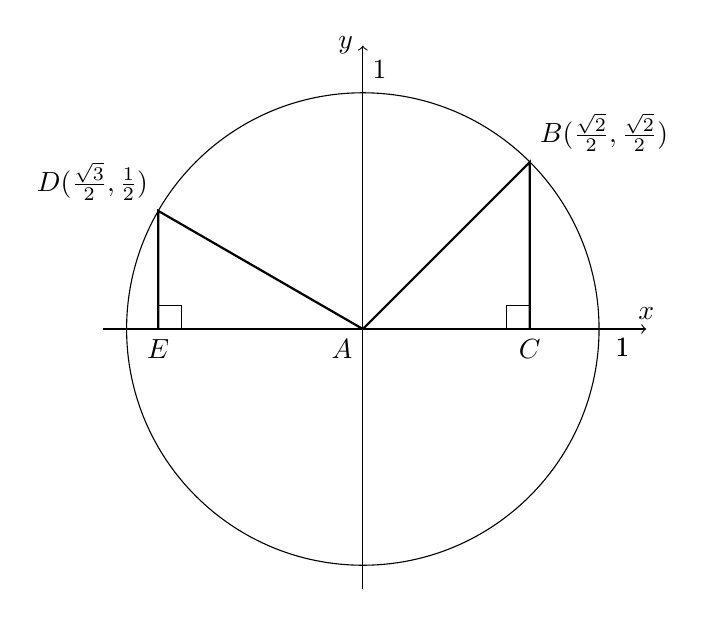
\begin{tikzpicture}[scale=3]
          \draw [->] (-1.1,0) -- (1.2,0) node [above] {$x$};
          \draw [->] (0,-1.1)--(0,1.2) node [left] {$y$};
          \draw (0,0) circle [radius=1];
          \node at (1.1,0)[below]{$1$};
          \node at (0,1.1)[right]{$1$};
          \draw [thick]
          (0,0)node[below left]{$A$}--
          (0.707,0.707)node[above right]{$B(\frac{\sqrt{2}}{2},\frac{\sqrt{2}}{2})$}--
          (0.707,0)node[below]{$C$};
          \draw (0.707,0)++(-0.1,0)--++(0,0.1)--+(0.1,0);
          \draw [thick]
          (0,0)--(-0.866,0.5)node[above left]{$D(\frac{\sqrt{3}}{2},\frac{1}{2})$}--
          (-0.866,0)node[below]{$E$};
          \draw (-0.866,0)++(0.1,0)--++(0,0.1)--+(-0.1,0);
          \node at (1.1,0)[below]{$1$};
          %\node at (3,2.6)[right]{$\sqrt{3}$};
          %\node at (1.3,2.5)[above]{$2$};
        \end{tikzpicture}
    \end{multicols} \vspace{1.5cm}

    \item Given two 30-60-90 degree triangles, $\triangle ABC \sim \triangle ADE$, with $BC=1$, $AC=\sqrt{3}$, $AB=2$. If $AD=6$ find the lengths of the other two sides.
      \begin{multicols}{2}
        \begin{enumerate}
        \item $DE=$
        \item $AE=$ \vspace{1cm}
      \end{enumerate}
        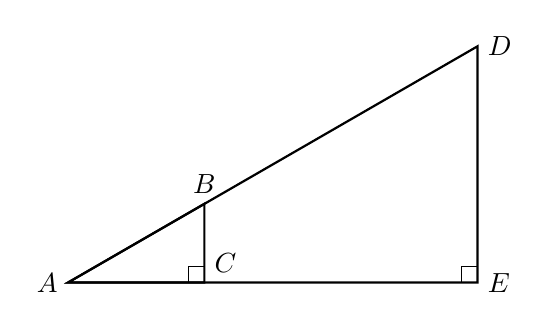
\begin{tikzpicture}[scale=1]
          \draw [thick]
          (0,0)node[left]{$A$}--
          (1.732,0)node[above right]{$C$}--
          (1.732,1)node[above]{$B$}--cycle;
          \draw (1.732,0)++(-0.2,0)--++(0,0.2)--+(0.2,0);
          \draw [thick]
          (0,0)--(5.2,0)node[right]{$E$}--
          (5.2,3)node[right]{$D$}--cycle;
          \draw (5.2,0)++(-0.2,0)--++(0,0.2)--+(0.2,0);
          %\node at (1.5,0)[below]{$1$};
          %\node at (3,2.6)[right]{$\sqrt{3}$};
          %\node at (1.3,2.5)[above]{$2$};
        \end{tikzpicture}
      \end{multicols}
      


    \item Simplify. Rationalize denominators.
    \begin{enumerate}
      \begin{multicols}{3}
        \item $\sqrt {72}$
        \item $\sqrt {50} - 4\sqrt{2}$
        \item $\displaystyle \frac{5}{\sqrt{5}}$
      \end{multicols}
      \end{enumerate}

\end{enumerate}
\end{document}

